\section{问题二的建模与求解：BMI 分组与最佳 NIPT 时点}

\subsection{达标时间估计}

NIPT 结果可靠的充要条件是 Y 染色体浓度达到阈值 $\theta=4\%$。因此每名孕妇存在一个``最早达标时间'' $t_i$，即其 Y 浓度首次达到 $4\%$ 的孕周。由问题一，Y 浓度随孕周的固定效应斜率为 $\beta_1=0.00319$（周$^{-1}$）。对第 $i$ 名孕妇，估计其个体浓度水平

\begin{equation}
  a_i=\frac{1}{n_i}\sum_{j=1}^{n_i}\big(Y_{ij}-\beta_1 t_{ij}\big),
\end{equation}

则个体达标时间为

\begin{equation}
  t_i=\frac{\theta-a_i}{\beta_1}.
\end{equation}

该估计方法用全体样本估计的共享斜率 $\beta_1$ 保证稳健性，用个体水平 $a_i$ 保留个体差异，避免了少数采样点直接回归导致的数值不稳定。

\subsection{达标时间与 BMI 的关系}

对 267 名孕妇的达标时间与 BMI 做回归，得到：

\begin{equation}
  t_i=-19.46+0.757\,B_i,
\end{equation}

回归系数 $0.757$ 在 $p<0.001$ 水平上显著（$t=4.02$），即 BMI 每升高 1，达标时间平均推迟约 $0.76$ 周，验证了题面``BMI 是影响最早达标时间主要因素''的判断。达标时间随 BMI 的分布如图~\ref{fig:q2_scatter} 所示。

\begin{figure}[H]
  \centering
  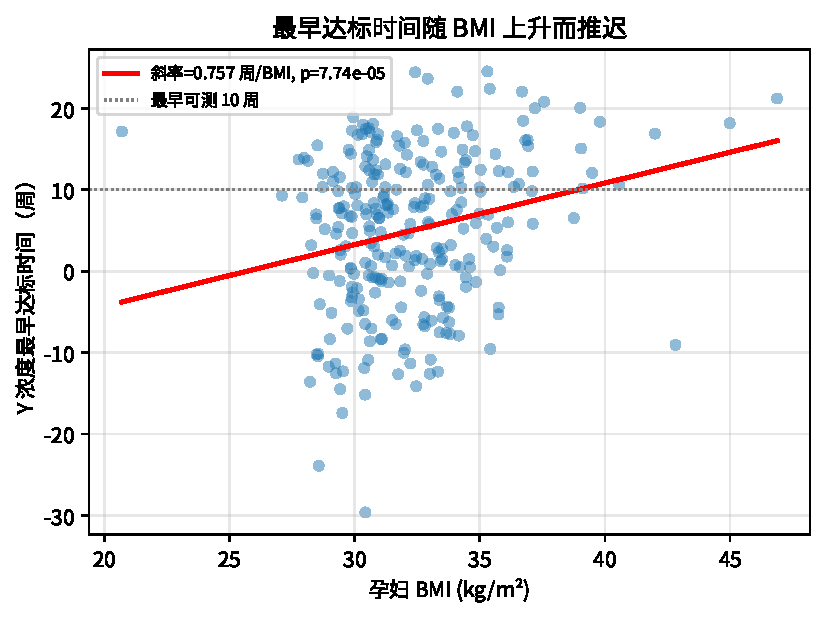
\includegraphics[width=0.62\textwidth]{../figures/fig2_1_attainment_vs_bmi.pdf}
  \caption{最早达标时间随 BMI 上升而推迟}
  \label{fig:q2_scatter}
\end{figure}

\subsection{BMI 合理分组与最佳时点}

按题面示例区间将孕妇分为五组，对每组取``组内 90\% 孕妇可靠达标''的最早时点作为最佳时点：该时点早于它则仍有较多孕妇 Y 浓度未达 $4\%$（结果不可靠），晚于它则治疗窗口进一步缩短（风险上升），故该时点兼顾检测可靠性与早检要求，使潜在风险最小。

\begin{center}
\begin{tabular}{ccccc}
\toprule
\textbf{BMI 区间} & \textbf{孕妇数} & \textbf{BMI 均值} & \textbf{最佳时点} & \textbf{风险等级} \\
\midrule
$[20,28)$ & 5 & 26.3 & 15.9 周 & 高风险（中期） \\
$[28,32)$ & 136 & 30.2 & 15.5 周 & 高风险（中期） \\
$[32,36)$ & 99 & 33.7 & 16.1 周 & 高风险（中期） \\
$[36,40)$ & 22 & 37.4 & 20.1 周 & 高风险（中期） \\
$\ge 40$ & 5 & 43.5 & 20.0 周 & 高风险（中期） \\
\bottomrule
\end{tabular}
\captionof{table}{各 BMI 组的最佳 NIPT 时点}
\label{tab:q2}
\end{center}

由表~\ref{tab:q2}，在样本充足的中部三组中，最佳时点随 BMI 升高由约 15.5 周推迟到约 20 周，趋势清晰（$[20,28)$ 与 $\ge 40$ 组样本过少，估计稳定性较低）。各组最佳时点如图~\ref{fig:q2_opt} 所示。

\begin{figure}[H]
  \centering
  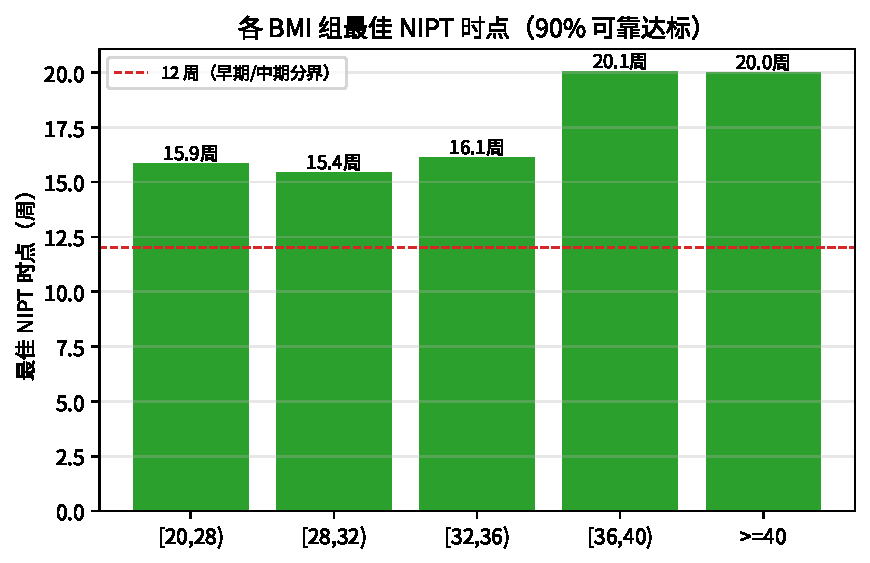
\includegraphics[width=0.68\textwidth]{../figures/fig2_2_optimal_timing.pdf}
  \caption{各 BMI 组最佳 NIPT 时点}
  \label{fig:q2_opt}
\end{figure}

\subsection{检测误差的影响}

检测误差 $\sigma_e$ 会使个体达标时间产生 $\sigma_e/\beta_1$ 的不确定性。为保证 90\% 可靠达标，最佳时点需后移约 $1.2816\,\sigma_e/\beta_1$ 周。取问题一混合模型残差标准差 $\sigma_e=0.0173$，则最佳时点需后移约 7.0 周；误差与后移量的关系如表~\ref{tab:q2_err} 与图~\ref{fig:q2_err} 所示。

\begin{center}
\begin{tabular}{ccccc}
\toprule
\textbf{检测误差} $\sigma_e$ & 0.005 & 0.010 & 0.0173 & 0.020 \\
\midrule
\textbf{最佳时点后移（周）} & 2.0 & 4.0 & 7.0 & 8.0 \\
\bottomrule
\end{tabular}
\captionof{table}{检测误差对最佳时点的推迟效应}
\label{tab:q2_err}
\end{center}

\begin{figure}[H]
  \centering
  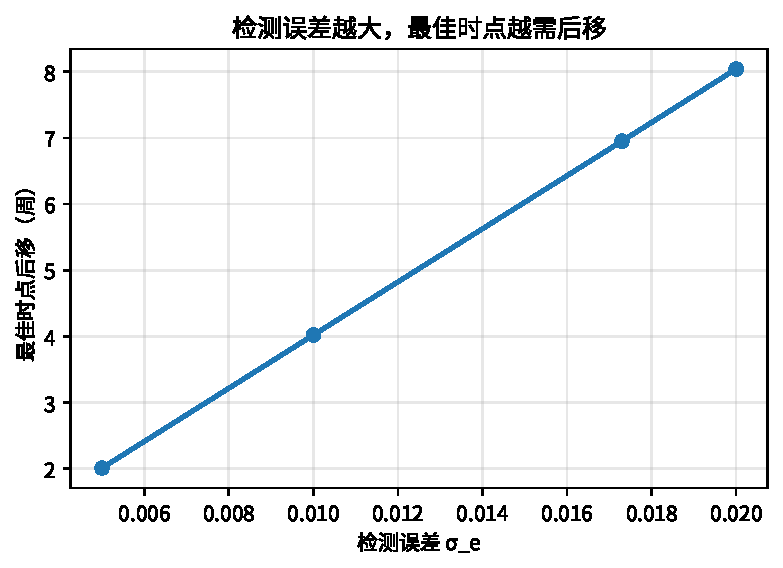
\includegraphics[width=0.6\textwidth]{../figures/fig2_3_error_sensitivity.pdf}
  \caption{检测误差越大，最佳时点越需后移}
  \label{fig:q2_err}
\end{figure}

可见检测误差对最佳时点影响显著：误差每增加约 0.005，最佳时点后移约 2 周。因此临床中控制检测精度对确定合适的 NIPT 时点至关重要。

问题二的求解流程如图~\ref{fig:flow_opt} 所示。

\begin{figure}[H]
  \centering
  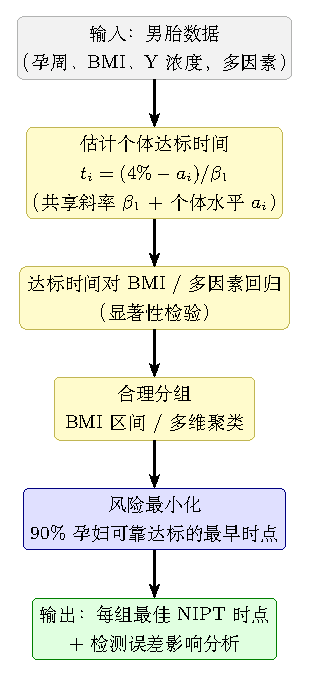
\includegraphics[width=0.75\textwidth]{../figures/fig_flow_optimal.pdf}
  \caption{BMI 分组与最佳 NIPT 时点求解流程}
  \label{fig:flow_opt}
\end{figure}
